
\chapter{Conclusions and perspectives\label{chap:Conclusion-and-perspective}}

\addcontentsline{lof}{chapter}{Conclusions and perspectives \lofpost}
%\addcontentsline{lot}{chapter}{Conclusions and perspectives\lofpost}

\singlespacing 
\epigraph{
Technological forecasting is even harder than weather forecasting.}
{Rolf Landauer} 
\doublespacing  \noindent 


\section{Conclusions}

In conclusion, we experimentally demonstrated that, despite the fundamental
indeterminism of quantum physics in the context of the monitoring
of the evolution of a system, it is possible to detect an advance
warning that signals the occurrence of an event, the quantum jump
from the ground state ($\G$) to the excited state $(\D)$ of a three-level
superconducting atom, prior to its complete occurrence (Sec.~\ref{sec:Catching-the-quantum}).
While the quantum jump begins at a random time and can be prematurely
interrupted by a click, a quantum jumps that completes follows a \emph{continuous},
\emph{deterministic}, and \emph{coherent} ``flight,'' which comes
as a surprise in view of standard textbooks on quantum mechanics.
The special nature of the transition was exploited to catch the jump
and reverse it to the ground state, $\G$. Additionally, the state
of the atom was tomographically reconstructed, $\rho_{c}$, as a function
of the duration of the catch signal, $\Delta t_{\mathrm{catch}}$,
from $6.8\times10^{6}$ individual experimental realizations, each
catching a single jump occurring at a random time. At the mid-flight
time of the quantum jump, $\Delta t_{{\rm mid}}$, the atom was observed
to be in coherent superposition of $\G$ (equivalent to no jump) and
$\D$ (equivalent to a jump), with state purity $\Tr{\rho_{c}^{2}}=0.75\pm0.004$.
Even when conditionally turning off the Rabi drive between $\G$ and
$\D$, $\Odg$, at the beginning of the jump, $\Delta t_{\mathrm{on}}=2\ \mathrm{\mu s}$,
the flight of the quantum jump was observed to nonetheless proceed
in coherent, deterministic, and essentially identical manner, despite
the absence of the coherent Rabi drive. This demonstrated  that the
role of $\Omega_{\mathrm{DG}}$ is to initiate the jump and set its
phase but is otherwise unimportant, and that the dynamics of the flight
are (essentially) entirely governed by the measurement-backaction
force due to the measurement, discussed in Chapter~\ref{chap:theoretical-description-jumps}. 

The jump coherence and deterministic-like character (any two jumps
take the same gradual flight) provide a small island of predictability
in a sea of uncertainty that was exploited, see Sec.~\ref{sec:Reversing-the-quantum},
to reverse the quantum jump to the ground state, thus precluding its
occurrence. When applied at the mid-flight time, $\Delta t_{\mathrm{mid}}$,
the protocol succeeded in reversing the jump to $\G$ with $82.0\%\pm0.3\%$
fidelity. Remarkably, under ideal conditions, every jump that would
complete is detected by the warning signal and reversed, thus eliminating
\emph{all} quantum jumps from $\G$ to $\D$, and preventing the atom
from ever reaching $\D$. Jumps that would not complete and are reversed
by the protocol meet their fate faster by the warning-based intervention.

In Sec.~\ref{subsec:Comparison-between-theory}, we showed that the
experimental results agree essentially without adjustable parameters
with the theory predictions, accounting for known experimental imperfections,
such as finite quantum measurement efficiency, $\eta$, temperature,
$n_{\mathrm{th}},$ dephasing mechanisms, $T_{1}$ and $T_{2}$, etc.
The agreement testifies for the validity, reliability, and predictive
power of quantum trajectory theory and suggests its critical role
in the practical development of real-time feedback techniques for
quantum system control. 

On a technological level, we developed a three-level superconducting
atom with distinct features of interest. By decoupling one of the
states, $\D$, from both the readout cavity and the environment, we
demonstrated a protected qubit design with notable quantum coherence,
$T_{\mathrm{2R}}^{\mathrm{D}}=120\pm5\,\mathrm{\mu s}$, importantly,
\emph{without }sacrificing measurement efficiency or speed, as typically
necessitated when decoupling a level, see Sec.~\ref{sec:circuit-design}.
Integral to the implementation was the design optimization with the
energy participation ratio (EPR) approach, as described in Sec.~\ref{sec:circuit-design}.
In Sec.~\ref{subsec:Measurement-induced-relaxation}, we demonstrated
the ability to populate the readout cavity with a large number of
photons without degrading the coherence properties of $\D$ due to
measurement-induced relaxation, $T_{1}\left(\bar{n}\right)$ . 

 

 


\section{Perspectives}

In the following, we discuss a few possible research directions that
build on the catch and reverse experiment and the development of the
Darkmon system, listed in ascending order of difficulty. 

\paragraph{Fundamental tests. }

The Darkmon three-level atom is a particularly versatile platform
for fundamental tests in quantum physics. Two unique aspects of the
$\B$/not-$\B$ measurement are important for fundamental tests: i)
it is information-asymmetric, and ii) its is degenerate. For definitiveness,
consider the situation where a measurement is performed on the atom
prepared in an unknown initial state. At first, the observer has no
knowledge of the system, i..e, zero bits of information. Performing
a measurement and obtaining a B outcome, the observer learns that
the measurement has projected the atom in the definite, pure state
$\B$, and now posses complete knowledge of the system, and has thus
gained $\mathcal{I}=\ln_{2}3\approx1.6$~bits of information, although
the initial state  remains unknown. In contrast, in obtaining a not-B
outcome, only $\mathcal{I}=\ln_{2}\left(3/2\right)\approx0.6$~bits
of information are gained, since the atom could still be in $\G$
or $\D$. The measurement has left behind 1~bit of the initial-state
information. Importantly, the $\B$/not-$\B$ measurement does not
disturb this bit, and preserves its quantum coherence. Since it leaves
behind a manifold of states untouched, it is known as \emph{degenerate
measurement.}

\emph{Contextuality.} — Degenerate measurements  are required to
perform tests of Kochen-Specker contextuality \citep{KochenSpecker1967},
which reveals an essential aspect of the nonclassical nature of quantum
measurements and constrains hidden variable theories; it can be viewed
as a complement to Bell's theorem. It follows from the degenerate
measurement requirement that a qutrit is the simplest system in which
contextuality can be observed, and the Darkmon system with its notable
control and coherence properties could prove a well-suited testbed
for rigorous tests \citep{Mermin1993-rev,Klyachko2008,Yu2012,Szangolies2015-book}.

\emph{Wavefunction collapse and the arrow of time. }— There is a growing
interest in the community to experimentally investigate the dynamics
of the wavefunction ``collapse'' \citep{Katz2006,Katz2008,Murch2013a,Hatridge2013,Weber2014,Campagne-Ibarcq2014,Campagne2016-Fluorescence,Jordan2016-fluorescence,Naghiloo2016,Tan2017,Harrington2017}
and associated fundamental questions. An interesting research direction
is to investigate the emergence of the apparent irreversibility of
the collapse, which, it is argued, yields the arrow of time in quantum
physics. Recently, theoretical work has emerged that suggests ways
in which quantum trajectory experiments can begin to probe this outstanding
question regarding the origin of the arrow of time with the tools
of quantum trajectory theory \citep{Dressel2017-arrow-of-time,Jordan2017-Janus}.
Focus so far has been almost exclusively on two level systems, but
important fundamental features in quantum physics, such as Kochen-Specker
contextuality, only emerge in systems of larger than two dimension.
The arrow of time is an especially interesting direction in view of
the results presented here, where we reverse quantum jumps prior to
their complete occurrence. We believe the Darkmon system and its degenerate
measurement could offer a unique vantage point on the problem. 

\emph{Thermodynamics.} — In a related research direction, the Darkmon
system could be employed to probe the emergence of thermodynamics
in continuously monitored systems, a question of active research in
the community. Specifically, understanding (and formulating) the fundamental
laws of thermodynamics in the quantum domain, as well as notions such
as work, heat, and Maxwell's demon, with applications to heat engines,
are under investigation and can be explored with quantum trajectories
in the multi-level system \citep{Alonso2016-thermo,Naghiloo2017-thermo,Elouard2017,Cottet2017}. 


\paragraph{Protected qubit with faithful readout. }

Technologically, pursuing further the ideas demonstrated with the
Darkmon system could lead to improved qubit coherences and measurement
capabilities within the cQED architecture with the aim of addressing
the third and fourth DiVincenzo criteria for practical quantum computation
\citep{DiVincenzo2000-criteria} . 

In the development of fast and high-fidelity superconducting qubit
readout, a number of non-linear process have been employed \citep{cooper2004,Astafiev2004-readout,Siddiqi2006,Lupascu2006-readout,Mallet2009-readout,Reed2010-readout},
but the linear dispersive readout, by means of a low-Q cavity \citep{Wallraff2005-readout,Blais2004,Johnson2012-readout,Riste2012-readout},
is adopted most widely. While the cavity inhibits the spontaneous
relaxation of the qubit, it introduces three additional loss mechanisms:
i) energy relaxation ($T_{1}$) due to the Purcell effect \citep{Esteve1986,Koch2007,Neeley2008-Purcell},
ii) qubit dephasing ($T_{\phi}$) due to the photon shot noise of
the readout cavity \citep{Blais2004,Schuster2005-ACStark,Gambetta2006-dephasing,Schuster2007,Gambetta2008-qm-traj,Sears2012-PhotonShot,Rigetti2012},
often dominated by residual thermal population, $n_{\mathrm{th}}$,
and iii) measurement-induced qubit energy relaxation ($T_{1}\left(\bar{n}\right)$)
\citep{Boissonneault2009-Photon-induced-relax,Slichter2012,Sank2016-T1vsNbar,Slichter2016-T1vsNbar}.
In contrast, the GD qubit in the Darkmon device is decoupled from
all three dissipation channels, while still benefiting from the cavity
properties, and not sacrificing the ability to perform a fast readout
or to monitor the atom continuously. Practically advantageous is that
the design is hardware-efficient (simple) in the sense that it does
not require additional control gates, such as fast-flux lines or DC
gates, or other high-power pump tones. 

An interesting idea to pursue further stems from the use of the readout
cavity in the catch and reverse experiment to provide amplification
(and transduction) of the $\B$ signal \emph{prior to} its transmission
to the following quantum-limited amplifier. Reducing losses in the
transmission, $\eta$, is an outstanding challenge in the field. However,
a strategy to overcome this problem is indicated by the design: the
addition of a built-in gain element at the site of the sample that
provides sufficient amplification to overcome transmission losses
and whose coupling to the readout signal can be tuned independently
of the gain (in the experiment, by means of $\Obg$). First, we note
that direct monitoring of the $\B$ signal, by means of fluorescence
detection, would have prohibited the faithful execution of the catch
and reverse protocol, since a large number of the click signals would
have been lost in transmission, due to $\eta$. In contrast, in the
experiment, the $\B$/not-$\B$ signal was effectively amplified fivefold
(with frequency transduction) by the readout scheme by use of the
large disperse shift, $\chi_{{\rm BC}}\gg\kappa_{C}$, and the cavity
probe tone, $\bar{n}$. In contrast to the usual dispersive readout
scheme, where the use of a large probe signal, $\bar{n},$ results
in degradation of the signal-to-noise ratio and qubit coherence due
to the $T_{1}\left(\bar{n}\right)$ effect, the $\D$ level was shown
to be essentially immune to this, see Sec.~\ref{subsec:Measurement-induced-relaxation}.
This could provide the ability to use strong pump tones to activate
interesting non-linear interactions \citep{Mundhada2017,Mundhada2018}
without harming $\D$, and to implement a gain element or to couple
$\B$ to the readout cavity in a dissipation engineered manner. A
specific form of the latter would realize a coupling term proportional
to $\kb{\rm G}{\rm B}\left(\hat{a}+\hat{a}^{\dagger}\right)$, where
$\hat{a}$ is the cavity annihilation operator that would operate
as follows: if the atom is not-in-$\B$, the cavity is empty, otherwise,
as $\Obg$ steers the atom from $\G$ to $\B$, the cavity fills with
$\bar{n}\gg1$ photons and activates a strong dissipation channel
of $\B$ that repopulates $\G$ before $\B$ is ever appreciably populated.
Similar-in-spirit dissipation channels have been realized, e.g., with
the double-drive reset-of-population (DDROP) protocol \citep{Geerlings2013-reset}.
If sufficient gain is achieved, no quantum-limited amplifier is required,
and the scheme would simplify the setup and  transmission losses,
$\eta$. 


\paragraph{Distillation and single-photon detector. }

The degenerate measurement of the Darkmon atom, perhaps employed
with the lowest four levels, could make it an interesting candidate
for magic-state and entanglement distillation protocols \citep{Bennett1996,Bravyi2005}.
Interestingly, the detection of a quantum jump from $\G$ to $\D$
can be viewed as the absorption and detection of a photon from the
input-output transmission line. In this sense, the three-level monitoring
scheme implements a photodetection apparatus for single flying microwave
photons in cQED. The device could be optimized with this goal in mind
to address the outstanding challenge of detecting itinerant microwave
photons with high efficiency \citep{Chen2011-FlyingPhoton,Fan2014-photonFly,Inomata2016-FlyingPhoton,Narla2016}.
In contrast to previous work on this subject, which focused on operating
detectors in a time-gated mode, the Darkmon scheme affords the advantage
of time-resolved, time-continuous photodetection with gain. It is
possible these advantages can be exploited for catching and releasing
flying Fock states \citep{Kalb2017,Campagne2017-entangle2}.


\paragraph{Stochastic drive, $\Omega_{{\rm DG}}$, and reversal. }

Realizable with the current device, one could catch and reverse the
quantum jump from $\G$ to $\D$ in the presence of a stochastic drive
from $\G$ to $\D$, $\Omega_{\mathrm{DG}}\left(t\right)$. The stochastic
drive more realistically models the effect of the environment and
breaks the feature of identical jumps; i.e., any two jumps no longer
look identical. The phase of the mid-flight superposition between
$\G$ and $\D$ is determined by the details of the stochastic $\Odg$
phase during the initial period of the jump, $\deltatcatch\ll\Delta t_{\mathrm{mid}}.$
Nonetheless, our prediction is that if the phase fluctuations of $\Odg$
at the beginning of the jump are known, one could still successfully
reverse the jump mid-flight with the appropriate coherent intervention.
This could be implemented by generating $\Odg$ with the FPGA controller,
on the fly, and having the controller calculate the correct intervention
angles, $\left\{ \theta_{I}\left(\deltatcatch\right),\varphi_{I}\left(\deltatcatch\right)\right\} $.
The reverse could be studied as a function of the bandwidth of the
noisy signal, $\Omega_{\mathrm{DG}}$ (practically, this could be
made as large as 25~MHz), thus exploring the crossover from jump
dynamics due to deterministic forces and those of the environment,
perhaps shedding further light on decoherence and measurement irreversibility.

\paragraph{Phase-agnostic reversal and quantum error correction.}

Calculation of the angles, $\left\{ \theta_{I}\left(\deltatcatch\right),\varphi_{I}\left(\deltatcatch\right)\right\} $,
becomes increasingly difficult for larger noise bandwidths. An alternative
strategy is to implement a phase-agnostic reversal. This could be
achieved with dissipation engineering \citep{Poyatos1996-qm-res-eng}
to conditionally dynamically cool to atom the ground state. Practical
cooling protocols have been experimentally demonstrated in cQED \citep{Valenzuela2006,Grajcar2008,Murch2012-bath-eng,Geerlings2013-reset,LiuYehan2016}. 

\begin{figure}
\begin{centering}
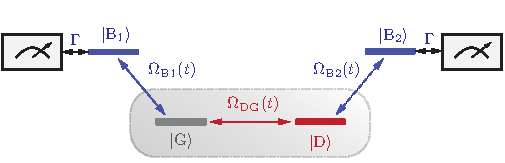
\includegraphics[scale=1.5]{conclusion/level4_diagram}
\par\end{centering}
\caption[Four-level atom with two counter-steering measurements]{\label{fig:4lvlatom}\textbf{Four-level atom with two counter-steering
measurements.} Sketch of a modified Darkmon atom consisting of four
levels: ground, $\G$, Dark, $\D$, a first ``Bright,'' $\ket{\mathrm{B}_{1}}$,
and a second ``Bright,'' $\ket{\mathrm{B}_{2}}$. Both Bright levels
are monitored at rate $\Gamma$, while controlled-actuated Rabi drives
$\Omega_{\mathrm{B1}}\left(t\right)$ and $\Omega_{\mathrm{B1}}\left(t\right)$
turn on the effective monitoring of $\G$ and $\D,$ respectively.
A potentially stochastic Rabi drive $\Omega_{\mathrm{DG}}\left(t\right)$
links $\G$ and $\D$.}
\end{figure}

Instead of dissipation engineering, the jump could be reversed by
means of a measurement-backaction force due to another measurement.
This will likely have to be probabilistic, unless adaptive measurements
\citep{Wiseman1995-adaptive,Jacobs2003-adaptive-msr} or measured-based
quantum steering is employed \citep{schrodinger1935gegenwartige,Murch2013a,Wiseman2007-steering}.
Specifically, we propose to investigate a four-level scheme that builds
on the Darkmon, see Fig.~\ref{fig:4lvlatom}. The ground state, $\G$,
is monitored though a Bright state, $\ket{\mathrm{B}_{1}}$, by means
of Rabi drive, $\Omega_{\mathrm{B1}}\left(t\right)$, and the photodetection
of $\ket{\mathrm{B}_{1}}$ at rate $\Gamma.$ Similarly, the Dark
level, $\D$, is monitored by coupling it with a Rabi drive $\Omega_{\mathrm{B2}}\left(t\right)$
to a second Bright state, $\ket{\mathrm{B}_{2}}$, monitored at rate
$\Gamma.$ Conditioned on no clicks, the $\G$ measurement steers
the atom toward $\D,$ see Chapter~\ref{chap:theoretical-description-jumps}.
In contrast, conditioned on no clicks, the $\D$ measurement steers
the atom toward $\G$. Both forces are phase agnostic. Since they
oppose each other, one can be used to undo the effect of the other
with proper conditioning and control of the Rabi drives. If $\G$
is measured subject to the Dark Rabi drive $\Odg$ from $\G$ to $\D$,
which could be deterministic or stochastic, while $\Omega_{\mathrm{B2}}=0$,
the protocol demonstrated in Chapter~1 is implemented. When the signal
warning of the occurrence of the quantum jump from $\G$ to $\D$
is detected, $\Omega_{\mathrm{B1}}$ is shut off. If the catch time
is set to $\Delta t_{\mathrm{mid}}$, the state of the GD superposition
is known to be on the GD equator, but its phase may be unknown. If
$\Omega_{\mathrm{B2}}$ is turned on and the record is conditioned
on no clicks, the jump should be reversed, no matter what the superposition
phase is. More generally, the opposition of the two counter-steering
no-click measurements offers a unique testbed for studying non-commuting
simultaneous measurements, a topic of rising interest in the field
\citep{Jordan2005-non-coom,Ruskov2010,Hacohen-Gourgy2016-non-comm,Perarnau-Llobet2017,Atalaya2017,Lewalle2017,Patti2017,Ficheux2017,Chantasri2018}. 

Quantum jumps are intimately involved in the detection and correction
of errors in quantum information systems \citep{Sun2013,Ofek2016}.
A controller continuously monitors an error syndrome, often parity,
such as that of a cavity state \citep{Ofek2016,Cohen2017-cw-parity-msr}
or multi-qubit stabilizer \citep{Huembeli2017}, and detects jumps
in the measurement record, which signal the occurrence of an error.
The error needs to corrected. Catch and reversing the quantum jump
of an error syndrome prior to its occurrence could prevent the error
from manifesting fully. A research direction that could be explored
is to couple the GD transition to the parity operator of a long-lived
quantum-memory cavity \citep{Kirchmair2013} that encodes a logical
quantum state \citep{Cochrane1999-catCode,Mirrahimi2014,Leghtas2015,Michael2016,LiLinshu2017,Touzard2017}.
The parity bit of the cavity state would be continuously mapped onto
the GD manifold. The state $\G$ would indicate \emph{no} error, while
$\D$ would indicate that an error has occurred. If the noise process
driving the parity bit flips has sufficiently narrow bandwidth, it
may be possible to extend the catch and reverse protocol to intervene
in the occurrence of the parity-bit error. By monitoring the $\B$/not-$\B$
measurement record as discussed in Chapter~1, the controller would
detect the advance-warning signal and immediately perform a phase-agnostic
reversal of the jump to prevent the error. Applications of the jump
reversal protocol to quantum error correction schemes present an interesting
and open direction for theoretical and experimental research. 

\paragraph{Closing statement. }

We hope the catch and reverse experiment offers a new vantage point
on the state-disturbing nature of measurements and the interplay between
deterministic forces and the necessarily-stochastic ones due to quantum
measurements. More generally, we hope it could provide a conceptually
simple but striking illustration to help write operationally-based,
rather than postulate-based, textbooks for quantum mechanics.

